%-----------------------------------To Be Updated for Classroom Examples--------------
%-------------------------------------------------------------------------------------
\documentclass{TMLSStyleGuideResumeVitae}
%------------------Style document from the Mathematical Learning Space style guide
\usepackage[english]{babel}
\usepackage{marginnote}
\usepackage{tikz}
\usepackage{hyperref}
\usetikzlibrary{positioning}
\usetikzlibrary{backgrounds}
\usepackage{tkz-berge}
\usepackage{sectsty}
\usepackage{aurical}
\usepackage[T1]{fontenc}
\fontsize{12}{15}
\sectionfont{\footnotesize}
\subsectionfont{\Large}
\subsubsectionfont{\large}
\paragraphfont{\lfootnotesize}
\usepackage{pagecolor}
\definecolor{c1}{rgb}{0.858, 0.188, 0.478}
\definecolor{c2}{RGB}{219, 48, 122}
\definecolor{c3}{cmyk}{0, 0.7808, 0.4429, 0.1412}
\definecolor{c4}{gray}{0.1}
\definecolor{c5}{RGB}{142, 68, 173}
\definecolor{blueish}{rgb}{0.565,0.886,1} 
\definecolor{greenish}{rgb}{0.565,1,0.886}
\definecolor{darkgray}{rgb}{0.15,0.15,0.15} 
\definecolor{lightgray}{rgb}{0.6,0.6,0.6}
\definecolor{shizen}{RGB}{242,246,246}
\graphicspath{{Figures/1/}}
\begin{document}
\pagecolor{shizen!1}	
%-------------------------------------------------------------------------------------------%
%----------------------------------------Contact Information--------------------------------%
%-------------------------------------------------------------------------------------------%
%-------------------------------------------------------------------------------------------%
\stringBox{\Fontskrivan\slshape\{Jeff Cromwell PhD}}
Linked In: https://www.linkedin.com/in/jeff-cromwellphd/

\section{Introduction}
\stringBox{\Fontskrivan\slshape\{Introduction goes here.}}
%-------------------------------------------------------------------------------------------%
%----------------------------------------Figure1--------------------------------------------% 
%-------------------------------------------------------------------------------------------%
\centering
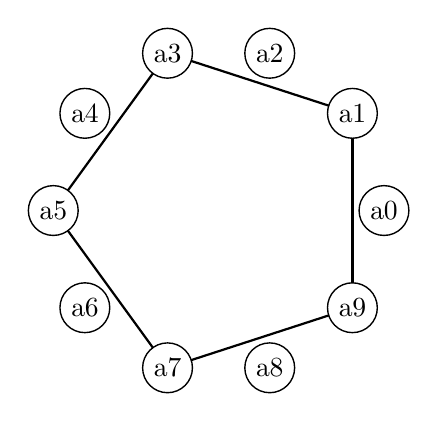
\begin{tikzpicture}[scale=0.35]
\grEmptyCycle[RA=6]{10}
\EdgeInGraphModLoop{a}{10}{2}{1}
\end{tikzpicture}
%-------------------------------------------------------------------------------------------%
%--------------------------------Summary----------------------------------------------------%
%-------------------------------------------------------------------------------------------%
\section{\centerline{\textcolor{c2}{Professional Summary}}}
%-------------------------------------------------------------------------------------------%
\stringBox{\Fontskrivan\slshape\{Academic and Professional Summary string goes here.}}
%\input{/Summary/ProfessionalSummaryAcademic}}
%-------------------------------------------------------------------------------------------%
%-------------------------------------------------------------------------------------------%
%----------------------------------------Jobs Section---------------------------------------%
%-------------------------------------------------------------------------------------------%
\section{Experience}
%---------------------------------------------------------------------------------------------------------------------------------%
%----------------------------Mathematical Learning Space--------------------------------------------------------------------------%
%---------------------------------------------------------------------------------------------------------------------------------%
\begin{enumerate}
\item {Weebly} {\href{http://mathlearningspace.weebly.com/}{\textcolor{c5}{Math Learning Space-Weebly}}}
\item {GitHib} {\href{https://github.com/MathematicalLearningSpace$}{ \textcolor{c5}{Mathematical Learning Space-GitHub}}}
\item {Math Numerical Projects}{ \textcolor{c2}{Development of the GitHub Mathematical Learning Space to Assist Students in Learning Applied Mathematics}}
\item {TMLS} {\href{http://mathlearningspace.weebly.com/}{Course 1: Differential Equations in Mathematical Biology, Botany, Chemistry and Oncology}}
\item {TMLS} {\href{http://mathlearningspace.weebly.com/}{Course 2: Design of Signal Transduction Networks of Molecular Interaction in Oncology Cell Lines}}
\item {TMLS} {\href{http://mathlearningspace.weebly.com/}{Course 3: Molecular Machine Learning with Topological Dynamics for Compound Discovery in Organelles}}
\item {TMLS} {\href{http://mathlearningspace.weebly.com/}{Course 4: Music and Mathematics Classical Music and Smooth Jazz Modeling, Analysis and Simulation}}
\end{enumerate}

%---------------------------------------------------------------------------------------------------%
%-------------------Selected Research and Teaching Positions----------------------------------------%
%---------------------------------------------------------------------------------------------------%

\section{University Research and Teaching Positions}
\stringBox{\Fontskrivan\slshape\{Figure Description goes here.}}
\begin{table}[H]
\small
\centering
\begin{tabular}{p{1cm}p{1cm}p{1cm}p{1cm}}
 \hline
 Year & University/Company & Location & Title & Comments \\ 
 \hline
2017 & Arizona State University -College of Health Solutions-Department of Biomedical Informatics & Tempe Arizona & Web Application Developer & \\
2016 & Wyzant & Tempe Arizona & Mathematics Tutor \\
2010-2011 & University of Pittsburgh - School of Medicine- Department of Biomedical Informatics & Pittsburgh Pa & Lecturer & Research Statistical Software Developer & \\
 \hline
\end{tabular}
\end{table}

%-------------------------------------------------------------------------------------------%
%----------------------------------------Education Section----------------------------------%
%-------------------------------------------------------------------------------------------%
\section{Education}
\stringBox{\Fontskrivan\slshape\{Figure Description goes here.}}

\begin{enumerate}
\item{2004}{Ph.D. Natural Resource Economics- \textcolor{c5}{Emphasis: Nonlinear Time Series Analysis and Chaos Theory}}{West Virginia University} 
\item{1998} {M.S. Agricultural Economics- \textcolor{c5}{Emphasis: Mathematical Statistics} }{West Virginia University}
\item{1986} {B.A. Economics- \textcolor{c5}{Emphasis: Mathematics and Philosophy} }{California University of PA}
\end{enumerate}

%-------------------------------------------------------------------------------------------%
%------------------------Lecture Posters and Programs Section-------------------------------%
%-------------------------------------------------------------------------------------------%
\section{Lectures and Articles}
\stringBox{\Fontskrivan\slshape\{In this section based on course 1 in the Mathematical Learning Space these examples are representations of articles from the courses.  Here the 3500 words 3 page 2 column data structure in XML,HTML and TeX with 3 tables and a 3 x 3 matrix of figures is the design pattern for scientific communication. Some have more than 3 tables and 9 figures.}}
%-------------------------------------------------------------------------------------------%
%-------------------------------Examples for Course 1---------------------------------------%
%-------------------------------------------------------------------------------------------%
\subsection{Course 1: Differential Equations in Mathematical Biology, Botany, Chemistry and Oncology}

\begin{enumerate}
\item \href{http://mathlearningspace.weebly.com/course-1.html}{\textcolor{c5}{Classroom Lecture 1-3 Topics: ODE, PDE, DDE}}}
\item Classroom Lecture 4-6 Topics: Fractional and Stochastic Calculus
\item Classroom Lecture 7-9 Topics: Stochastic Differential Equations
\item Classroom Lecture 10-12 Topics: Nonlinear Time Series Models
\item Classroom Lecture 13-15 Topics: Markov Models
\item Classroom Lecture 16-18 Topics: Optimization
\item Classroom Lecture 19-21 Topics: GA and DE Algorithms and Fitness Metric
\item Classroom Lecture 22-24 Topics: Topology Dynamics and Equilibrium
\item Classroom Lecture 25-27 Topics: Phase Space, Global and Local Stability
\item Classroom Lecture 28-30 Topics: Application Study 1,2,3
\end{enumerate}

%-------------------------------------------------------------------------------------------%
%-------------------------------------------------------------------------------------------%
%-------------------------------------------------------------------------------------------%
\subsubsection{Conference Posters from Course 1}
\begin{enumerate}
\item \href{}{\textcolor{c5}{Classroom Lecture 1-3 Topics:}}}
\item \href{}{\textcolor{c5}{Classroom Lecture 4-6 Topics:}}}
\item \href{}{\textcolor{c5}{Classroom Lecture 7-9 Topics: A Design Pattern for Stochastic Volatility and Stochastic Differential Equation Models Applied To Foreign Exchange Rate Markets}}}
\item \href{}{\textcolor{c5}{Classroom Lecture 10-12 Topics:}}}
\item \href{}{\textcolor{c5}{Classroom Lecture 13-15 Topics:}}}
\item \href{}{\textcolor{c5}{Classroom Lecture 16-18 Topics:}}}
\item \href{}{\textcolor{c5}{Classroom Lecture 19-21 Topics:}}}
\item \href{}{\textcolor{c5}{Classroom Lecture 22-24 Topics:}}}
\item \href{}{\textcolor{c5}{Classroom Lecture 25-27 Topics:}}}
\item \href{}{\textcolor{c5}{Classroom Lecture 28-30 Topics:}}}
\end{enumerate}

%-------------------------------------------------------------------------------------------%
%-------------------------------------------------------------------------------------------%
%-------------------------------------------------------------------------------------------%
\subsubsection{Journal Articles from Course 1}
%-------------------------------------------------------------------------------------------%
\stringBox{\Fontskrivan\slshape\{These journal articles are in the process of review for journal submission.  If you would like to review an article or collection of articles before publication, please send a note on the article(s) selected with the form on the mathematical learning space web site.}}
\begin{enumerate}
\item Lecture 1-3 Article: \href{}{DRAFT Sample: DNA Shape Categories for Statistical Learning Models of Gene Overexpression, Amplification, Mutation and Regulation in GastroIntestinal Cancer}
\item Lecture 4-6 Article: \href{}{DRAFT Sample: Delayed Differential Equations for Intestinal Metaplasia of Gene Expression Modulation in Gastric Cancer}
\item Lecture 7-9 Article: \href{}{DRAFT Sample: Mucomodulators and Mucin Dependent Oncogenic cell Signaling and Immunomodulation in Gastric Cancer}
\item Lecture 10-12 Article: \href{}{DRAFT Sample: A Mathematical Model of Molecular Complexity and Epigenetic Modifications with Mucin Regulation in GastroIntestinal Cancers}
\item Lecture 13-15 Article: \href{}{DRAFT Sample: Minimal Spanning Trees and Multivariate Nonparametric Distributional Testing for Gastric Cancer Chemosensitivity}
\item Lecture 16-18 Article: \href{}{DRAFT Sample: A Mathematical Model of Multi-functional Regulators of Gut Homeostasis with Microbiota Diversity}
\item Lecture 19-21 Article: \href{}{DRAFT Sample: Differential Equation Specification and Polysyllabic Filtering for Medical and Chemical Vocabulary Interaction Models in GastroIntestinal Cancer Research}
\item Lecture 22-24 Article: \href{}{DRAFT Sample: Stability Classification Designs for Differential Equation Systems of DNA, Protein and Compound Interaction Combinatorics}
\item Lecture 25-27 Article: \href{}{DRAFT Sample: A Delayed Differential Equation Model of Phytochemicals in GastroIntestinal Cancers}
\item Lecture 28-30 Article: \href{}{DRAFT Sample: Delayed Fractional Differential Equation Models in Gastrointestinal Cancers}
\end{enumerate}
%-------------------------------------------------------------------------------------------%
%-------------------------------Examples for Course 2---------------------------------------%
%-------------------------------------------------------------------------------------------%
\subsection{Course 2: Design of Signal Transduction Networks of Molecular Interaction in Oncology Cell Lines}
%-------------------------------------------------------------------------------------------%
\begin{enumerate}
\item \href{http://mathlearningspace.weebly.com/course-2.html}{\textcolor{c5}{Classroom Lecture 1-3 Topics: KEGG Review}}}
\item Classroom Lecture 4-6 Topics:  Signal Transduction and QSAR
\item Classroom Lecture 7-9 Topics: Botany 1 and 2 Shikimate
\item Classroom Lecture 10-12 Topics: MAPK, Calcium cAMP
\item Classroom Lecture 13-15 Topics: Fox0 Cell cycle mTor
\item Classroom Lecture 16-18 Topics: Longevity Immune System Wnt Notch Hedgehog TGF-Beta and VGF
\item Classroom Lecture 19-21 Topics: Apelin Hippo JakStat Insulin WDR
\item Classroom Lecture 22-24 Topics:  Digestion I and II Sugar and Insulin
\item Classroom Lecture 25-27 Topics:  Metabolism Obesity Pancreatic Signalling I
\item Classroom Lecture 28-30 Topics:  Application Study I and II
\end{enumerate}
%-------------------------------------------------------------------------------------------%
%-------------------------------------------------------------------------------------------%
%-------------------------------------------------------------------------------------------%
\subsubsection{Conference Posters from Course 2}
\begin{enumerate}
\item \href{}{\textcolor{c5}{Classroom Lecture 1-3 Topics:}}}
\item \href{}{\textcolor{c5}{Classroom Lecture 4-6 Topics:}}}
\item \href{}{\textcolor{c5}{Classroom Lecture 7-9 Topics:}}}
\item \href{}{\textcolor{c5}{Classroom Lecture 10-12 Topics:}}}
\item \href{}{\textcolor{c5}{Classroom Lecture 13-15 Topics:}}}
\item \href{}{\textcolor{c5}{Classroom Lecture 16-18 Topics:}}}
\item \href{}{\textcolor{c5}{Classroom Lecture 19-21 Topics:}}}
\item \href{}{\textcolor{c5}{Classroom Lecture 22-24 Topics:}}}
\item \href{}{\textcolor{c5}{Classroom Lecture 25-27 Topics:}}}
\item \href{}{\textcolor{c5}{Classroom Lecture 28-30 Topics:}}}
\end{enumerate}
%-------------------------------------------------------------------------------------------%
%-------------------------------------------------------------------------------------------%
%-------------------------------------------------------------------------------------------%
\subsubsection{Journal Articles from Course 2}
%-------------------------------------------------------------------------------------------%
\stringBox{\Fontskrivan\slshape\{These journal articles are in the process of review for journal submission.  If you would like to review an article or collection of articles before publication, please send a note on the article(s) selected with the form on the mathematical learning space web site.}}
\begin{enumerate}
\item Lecture 1-3 Article: \href{}{DRAFT Sample: A Mathematical model of Cell Cycle Process Regulation of Cell Cycle, Chromosome Segregation and G2/M Transition}
\item Lecture 4-6 Article: \href{}{DRAFT Sample: A Mathematical Model of Teleomere Maintenance and Telomeric DNA Binding}
\item Lecture 7-9 Article: \href{}{DRAFT Sample: A Mathematical Model of Mitotic Biological Processes in a Gene Ontology}
\item Lecture 10-12 Article: \href{}{DRAFT Sample: A Mathematical Model of DNA Repair Genes/Proteins Based on Molecular Function
and Signaling Pathway}
\item Lecture 13-15 Article: \href{}{DRAFT Sample: A Mathematical Model of Glycoproteins of the Epithelia Mucosa in the Mucocilary System}
\item Lecture 16-18 Article: \href{}{DRAFT Sample: A Mathematical Model of Transcriptional Activity for Helix-Loop-Helix Proteins}
\item Lecture 19-21 Article: \href{}{DRAFT Sample: A Delay Differential Equation Model for Signal Transduction in Hepatocellular Carcinoma}
\item Lecture 22-24 Article: \href{}{DRAFT Sample: A Mathematical Model of Heterodimer DNA helix Bending}}
\item Lecture 25-27 Article: \href{}{DRAFT Sample: A Mathematical Model of the Regulation of Intracellular Signaling Cascades}
\item Lecture 28-30 Article: \href{}{DRAFT Sample: A Mathematical Model of Motif Mediation in the Heterotrimeric G-protein Signaling Pathway}
\end{enumerate}
%-------------------------------------------------------------------------------------------%
%-------------------------------Examples for Course 3---------------------------------------%
%-------------------------------------------------------------------------------------------%
\subsection{Course 3: Molecular Machine Learning with Topological Dynamics for Compound Discovery in Organelles}
\begin{enumerate}
\item \href{http://mathlearningspace.weebly.com/course-3.html}{\textcolor{c5}{Classroom Lecture 1-3 Topics: Ribosome ER Smooth and Rough}}}
\item Classroom Lecture 4-6 Topics:  Translation and Transcription Models
\item Classroom Lecture 7-9 Topics:  Normal Mode Analysis Compound Discovery QSAR Models
\item Classroom Lecture 10-12 Topics: WDR and G Quadruplexes Heat Shock Proteins
\item Classroom Lecture 13-15 Topics: Machine Learning Models I, II and III
\item Classroom Lecture 16-18 Topics:  Ribosome Model
\item Classroom Lecture 19-21 Topics: Chaperonin Model
\item Classroom Lecture 22-24 Topics: Proteasome Model
\item Classroom Lecture 25-27 Topics: Network Models Molecular Machines I and II
\item Classroom Lecture 28-30 Topics: Application Study I, II and III
\end{enumerate}

%-------------------------------------------------------------------------------------------%
%-------------------------------------------------------------------------------------------%
%-------------------------------------------------------------------------------------------%
\subsubsection{Conference Posters from Course 3}
\begin{enumerate}
\item \href{}{\textcolor{c5}{Classroom Lecture 1-3 Topics:}}}
\item \href{}{\textcolor{c5}{Classroom Lecture 4-6 Topics:}}}
\item \href{}{\textcolor{c5}{Classroom Lecture 7-9 Topics:}}}
\item \href{}{\textcolor{c5}{Classroom Lecture 10-12 Topics:}}}
\item \href{}{\textcolor{c5}{Classroom Lecture 13-15 Topics:}}}
\item \href{}{\textcolor{c5}{Classroom Lecture 16-18 Topics:}}}
\item \href{}{\textcolor{c5}{Classroom Lecture 19-21 Topics:}}}
\item \href{}{\textcolor{c5}{Classroom Lecture 22-24 Topics:}}}
\item \href{}{\textcolor{c5}{Classroom Lecture 25-27 Topics:}}}
\item \href{}{\textcolor{c5}{Classroom Lecture 28-30 Topics:}}}
\end{enumerate}

\subsubsection{Journal Articles from Course 3}
%-------------------------------------------------------------------------------------------%
\stringBox{\Fontskrivan\slshape\{These journal articles are in the process of review for journal submission.  If you would like to review an article or collection of articles before publication, please send a note on the article(s) selected with the form on the mathematical learning space web site.}}
\begin{enumerate}
\item Lecture 1-3 Article: \href{}{A Mathematical Model of Ribosome Flow}
\item Lecture 4-6 Article: \href{}{A Mathematical Model of Transcriptional, Translational, Protein Folding, and Post Translational Errors}
\item Lecture 7-9 Article: \href{}{A Mathematical Model of the Biosynthesis of Alkaloids from Shikimate Pathway}
\item Lecture 10-12 Article: \href{}{A Mathematical Model of WDR and G Quadruplexes}
\item Lecture 13-15 Article: \href{}{A QSAR Feature Matrix Design For Protein-Compound Interaction}
\item Lecture 16-18 Article: \href{}{A Mathematical Model of Ribosome Model with Circular mRNA}
\item Lecture 19-21 Article: \href{}{A Mathematical Model of Stress Induced Upregulation in Protein Responses}
\item Lecture 22-24 Article: \href{}{A Mathematical Model of the Assembly of a 20S Proteasome with Peptide Post-Translational Modification}
\item Lecture 25-27 Article: \href{}{A Molecular Machine Learning Algorithm of Multi-Protein Complexes in The Digestion System}
\item Lecture 28-30 Article: \href{}{A Mathematical Model of Normal Mode Superposition in Compound-Protein Interaction}
\end{enumerate}
%-------------------------------------------------------------------------------------------%
%-------------------------------Examples for Course 4---------------------------------------%
%-------------------------------------------------------------------------------------------%
\subsection{Course 4: Music and Mathematics Classical Music and Smooth Jazz Modeling, Analysis and Simulation}
%-------------------------------------------------------------------------------------------%
\begin{enumerate}
\item \href{http://mathlearningspace.weebly.com/course-4.html}{\textcolor{c5}{Classroom Lecture 1-3 Topics: Music Review}}}
\item Classroom Lecture 4-6 Topics: Music Sequences Classification Chord Classification
\item Classroom Lecture 7-9 Topics: Arrangements Polyphonic Melodies
\item Classroom Lecture 10-12 Topics: Wavelet Analysis Multiresolution analysis
\item Classroom Lecture 13-15 Topics: Harmonic Analysis
\item Classroom Lecture 16-18 Topics: Analysis of Modes
\item Classroom Lecture 19-21 Topics: Classical Music I, II and III
\item Classroom Lecture 22-24 Topics: Markov Models
\item Classroom Lecture 25-27 Topics: Composition Model I, II, and III
\item Classroom Lecture 28-30 Topics: Jazz Music I and II, Romantic Music I
\end{enumerate}

%-------------------------------------------------------------------------------------------%
%-------------------------------------------------------------------------------------------%
%-------------------------------------------------------------------------------------------%
\subsubsection{Conference Posters from Course 4}
\begin{enumerate}
\item \href{}{\textcolor{c5}{Classroom Lecture 1-3 Topics:}}}
\item \href{}{\textcolor{c5}{Classroom Lecture 4-6 Topics:}}}
\item \href{}{\textcolor{c5}{Classroom Lecture 7-9 Topics:}}}
\item \href{}{\textcolor{c5}{Classroom Lecture 10-12 Topics:}}}
\item \href{}{\textcolor{c5}{Classroom Lecture 13-15 Topics:}}}
\item \href{}{\textcolor{c5}{Classroom Lecture 16-18 Topics:}}}
\item \href{}{\textcolor{c5}{Classroom Lecture 19-21 Topics:}}}
\item \href{}{\textcolor{c5}{Classroom Lecture 22-24 Topics:}}}
\item \href{}{\textcolor{c5}{Classroom Lecture 25-27 Topics:}}}
\item \href{}{\textcolor{c5}{Classroom Lecture 28-30 Topics:}}}
\end{enumerate}
%-------------------------------------------------------------------------------------------%
%-------------------------------------------------------------------------------------------%
%-------------------------------------------------------------------------------------------%
\subsubsection{Journal Articles from Course 4}
%-------------------------------------------------------------------------------------------%
\stringBox{\Fontskrivan\slshape\{These journal articles are in the process of review for journal submission.  If you would like to review an article or collection of articles before publication, please send a note on the article(s) selected with the form on the mathematical learning space web site.}}
\begin{enumerate}
\item Lecture 1-3 Article: \href{https://github.com/MathematicalLearningSpace/Reading-Room-A/blob/master/Classroom%20Lecture%20Model%20Series_Course_4_Topic%201_Lecture_1_2_3_Journal_Article_1.tex}{DRAFT Sample: An Examination of Ratios and Spectral Properties for a Set of Non-Automated and Human Curated Genre Based Music Compositions}
\item Lecture 4-6 Article: \href{https://github.com/MathematicalLearningSpace/Reading-Room-A/blob/master/Classroom%20Lecture%20Model%20Series_Course_4_Topic%201_Lecture_4_5_6_Journal_Article_2.tex}{DRAFT Sample: Multivariate Distribution Analysis based on Moment Spectral Properties for a Contemporary Jazz Album}
\item Lecture 7-9 Article: \href{https://github.com/MathematicalLearningSpace/Reading-Room-A/blob/master/Classroom%20Lecture%20Model%20Series_Course_4_Topic%201_Lecture_7-8-9_Journal_Article_3.tex}{DRAFT Sample: Energy Tracking Operators for Amplitude and Frequency Modulation in Multi-Instrument Jazz Compositions}
\item Lecture 10-12 Article: \href{https://github.com/MathematicalLearningSpace/Reading-Room-A/blob/master/Classroom%20Lecture%20Model%20Series_Course_4_Topic%201_Lecture_10-11-12_Journal_Article_4.tex}{DRAFT Sample: Categorical Temporal Transformation Designs for Smoothing Models of Jazz Compositional Waveforms}
\item Lecture 13-15 Article: \href{https://github.com/MathematicalLearningSpace/Reading-Room-A/blob/master/Classroom%20Lecture%20Model%20Series_Course_4_Topic%201_Lecture_13_14_15_Journal_Article_5.tex}{DRAFT Sample: Spectra Comparisons and Q Resonance Factors for Music Compositions with Repeated Motif Designs for the Smooth Jazz Genre}
\item Lecture 16-18 Article: \href{https://github.com/MathematicalLearningSpace/Reading-Room-A/blob/master/Classroom%20Lecture%20Model%20Series_Course_4_Topic%201_Lecture_16-17-18_Journal_Article_6.tex}{DRAFT Sample: Change Point and Interval Designs For Music Composition Based on Repeated Motif Momemt Properties}
\item Lecture 19-21 Article: \href{https://github.com/MathematicalLearningSpace/Reading-Room-A/blob/master/Classroom%20Lecture%20Model%20Series_Course_4_Topic%201_Lecture_19_20_21_Journal_Article_7.tex}{DRAFT Sample: A Semi-Markovian Model of Octave Frequency Visitation and Note Distribution in One Minute Classical and Jazz Music Compositions}
\item Lecture 22-24 Article: \href{https://github.com/MathematicalLearningSpace/Reading-Room-A/blob/master/Classroom%20Lecture%20Model%20Series_Course_4_Topic%201_Lecture_22_23_24_Journal_Article_8.tex}{DRAFT Sample: Acoustic Complexity, Entropy and Curvature Ratio Designs for Solo, Duet, Trio and Quartet Instrumentation Variation of Musical Phrasing for Jazz Compositions}
\item Lecture 25-27 Article: \href{https://github.com/MathematicalLearningSpace/Reading-Room-A/blob/master/Classroom%20Lecture%20Model%20Series_Course_4_Topic%201_Lecture_25_26_27_Journal_Article_9.tex}{DRAFT Sample: Machine Learning of Waveform Mixing and Chord Sequences in Classical Music Compositions}
\item Lecture 28-30 Article: \href{https://github.com/MathematicalLearningSpace/Reading-Room-A/blob/master/Classroom%20Lecture%20Model%20Series_Course_4_Topic%201_Lecture_28_29_30_Journal_Article_10.tex}{DRAFT Sample: Music Chabot Interaction For Single and Multi-Minute Solo and Trio Classical and Jazz Music Album Designs for the Piano, Marimba and Guitar}
\end{enumerate}
%-------------------------------------------------------------------------------------------%
%-----------------------------------------Publications Section------------------------------%
%-------------------------------------------------------------------------------------------%
\section{Publications}
\stringBox{\Fontskrivan\slshape\{Current List of journals for publications.}}
\begin{table}[ht]
\footnotesize
\centering
\begin{tabular}{p{1cm}p{6cm}p{2cm}}
 \hline
 ID & Journal Name & State \\ 
 \hline
CMA & {\href{http://mathlearningspace.weebly.com/}{\textcolor{c5}{Computer and Mathematics with Applications}}} & In Development\\
AM & {\href{http://mathlearningspace.weebly.com/}{\textcolor{c2}{Discrete Applied Mathematics}}} & In Development \\
EM & {\href{http://mathlearningspace.weebly.com/}{\textcolor{c1}{Economic Modelling}}} & In Development \\
AML & {\href{http://mathlearningspace.weebly.com/}{\textcolor{c2}{Applied Mathematics Letters}}} & In Development\\
SPL & {\href{http://mathlearningspace.weebly.com/}{\textcolor{c3}{Statistics and Probability Letters}}} & In Development \\
NN & {\href{http://mathlearningspace.weebly.com/}{\textcolor{c4}{Neural Networks}}} & In Development\\
CSDA & {\href{http://mathlearningspace.weebly.com/}{\textcolor{c1}{Computational Statistics and Data Analysis}}} & In Development\\
IJMI & {\href{http://mathlearningspace.weebly.com/}{\textcolor{c5}{International Journal of Medical Informatics}}} & In Development\\
AIMS & {\href{http://mathlearningspace.weebly.com/}{\textcolor{c5}{AIM Mathematics Journal}}} & In Development\\
CLJ & {\href{http://mathlearningspace.weebly.com/}{\textcolor{c5}{Cancer Letter Journals}}} & In Development\\
MTS & {\href{http://mathlearningspace.weebly.com/}{\textcolor{c5}{Music Theory Spectrum}}} & In Development\\
IJC & {\href{http://mathlearningspace.weebly.com/}{\textcolor{c5}{Indian Journal of Cancer}}} & In Development\\
 \hline
\end{tabular}
\end{table}
%-------------------------------------------------------------------------------------------%
\begin{enumerate}
\item \textbf{Cancer Letter Series:}\textcolor{c4}{Title 1:}
\item \textbf{AIMS Mathematics Series:}{Title 1:}
\end{enumerate}

%-----------------------------------------------------------------------------------------------------------------------------------------%
%---------------------------------------Articles Examples---------------------------------------------------------------------------------%
%-----------------------------------------------------------------------------------------------------------------------------------------%

%--------------------------------------------------------------------------------------------------
%---------------Research Portfolio in Cancer Research for Summer Session I,II and Fall Semester 2019
%---------------------------------------------------------------------------------------------------
\section{\textcolor{black}{Research Article Portfolio in GastroIntestinal Cancer}}

\begin{table}[H]\footnotesize
\caption{Research Article Portfolio in GastroIntestinal Cancer less than 3500 Word Data Structure}	
\begin{tabular}{p{7cm}p{1cm}p{0.25cm}}
\hline
Title & Semester & \\   
\hline
\hline
\end{tabular}
\end{table}

\begin{enumerate}
\item Working Draft: A Mathematical Model of the PI3K-AKT-mTOR Cascade and Exosomal MicroRNAs with AntiMetabolites for Gastric Cancer
\end{enumerate}
%-------------------------------------------------------------------------------------------%
%------------------------------Music Research Compositions Section--------------------------%
%-------------------------------------------------------------------------------------------%
\section{Music Research Compositions}

\begin{enumerate}
\item \href{https://github.com/MathematicalLearningSpace/Music-Room-A/blob/master/Composition_1.xml}{Composition 1}
\item \href{https://github.com/MathematicalLearningSpace/Music-Room-A/blob/master/Composition_2.xml}{Composition 2}
\item \href{https://github.com/MathematicalLearningSpace/Music-Room-A/blob/master/Composition_3.xml}{Composition 3}
\item \href{https://github.com/MathematicalLearningSpace/Music-Room-A/blob/master/Composition_4.xml}{Composition 4}
\item \href{https://github.com/MathematicalLearningSpace/Music-Room-A/blob/master/Composition_5.xml}{Composition 5}
\item \href{https://github.com/MathematicalLearningSpace/Music-Room-A/blob/master/Composition_6.xml}{Composition 6}
\item \href{https://github.com/MathematicalLearningSpace/Music-Room-A/blob/master/Composition_7.xml}{Composition 7}
\item \href{https://github.com/MathematicalLearningSpace/Music-Room-A/blob/master/Composition_8.xml}{Composition 8}
\item \href{https://github.com/MathematicalLearningSpace/Music-Room-A/blob/master/Composition_9.xml}{Composition 9}
\item \href{https://github.com/MathematicalLearningSpace/Music-Room-A/blob/master/Composition_10.xml}{Composition 10}
\end{enumerate}

%-------------------------------------------------------------------------------------------%
%-----------------Scientific Visualization Portfolio Section--------------------------------%
%-------------------------------------------------------------------------------------------%
\section{Scientific Visualization Portfolio}
\stringBox{\Fontskrivan\slshape\{Figure Description goes here.}}
\begin{enumerate}
\item Diagram A \textcolor{c4}{Caption:}
\end{enumerate}
%-------------------------------------------------------------------------------------------%
%----------------Graphics Design:Article 1--------------------------------------------------%
%-------------------------------------------------------------------------------------------%
\footnotesize
\begin{figure}[h]
\centering
%\includegraphics[scale=0.2]{Figure3B.png}
\caption{\textcolor{c5}{\textbf{Classroom Lecture Model Series 1:}}\footnotesize  A Mathematical Model}
\label{fig:Figure1}
\end{figure}
%----------------------------------------------------------------------------------------------------------------------------------------%
%--------------------------------Graphics Design:Article Examples------------------------------------------------------------------------%
%----------------------------------------------------------------------------------------------------------------------------------------%
\stringBox{\Fontskrivan\slshape\{Figure Description goes here from the articles}}
\vspace{6pt}
\begin{figure}[h]
	\centering
	\begin{minipage}[b]{0.5\linewidth}
		%\includegraphics[scale=0.25]{Example_AIMS_1_Figure_4.png}
		\caption{\tiny Correlation Matrix of the solution paths from the Differential Equation system for LD, ATR, ATR phosphorylated , p21, p21CE, total p21, DDE2, and RB }
		\label{fig:networkA}
	\end{minipage}\hfill
	\begin{minipage}[b]{0.5\linewidth}
		%\includegraphics[scale=0.25]{Example_AIMS_2_Figure_8A.png}
		\caption{\tiny Intensity z-score for the expression of mTOR based on a collection of cell lines in the NCI-60 cancer data set }
		\label{fig:networkB}
	\end{minipage}\hfill
	\begin{minipage}[b]{0.5\linewidth}
		%\includegraphics[scale=0.25]{Example_AIMS_3_Figure_3.png}
		\caption{\tiny Realization paths of a three species stochastic differential equation system}
		\label{fig:networkC}
	\end{minipage}\hfill
	\begin{minipage}[b]{0.5\linewidth}
		%\includegraphics[scale=0.25]{Example_AIMS_5_Figure_6A.png}
		\caption{\tiny A weighted directed graph from machine learning algorithms composed in the C language }
		\label{fig:networkC}
	\end{minipage}\hfill
	\caption{\textcolor{c5}{\textbf{Classroom Lecture Model Series 5:}}\tiny  Allo-Artificial Intelligent Filtering Patterns with Stochastic Search Optimization for Recommender System Design and Molecular Machine Learning }
	\label{fig:Figure5}
\end{figure}
%-------------------------------------------------------------------------------------------%
%-------------------------------------------------------------------------------------------%
%-------------------------------------------------------------------------------------------%
\section{\textcolor{black}{A:Portfolio of Differential Equation Research}}

\testBox{\Fontskrivan\slshape{In Figure 1 from Course N Lecture N Article 1, Figure 2 displays from Course N Lecture N Article 2, Figure 3 is an example from Course N Lecture N Article 3,
Figure 4 is an example from Course N Lecture N Article 4, Figure 5 is an example from Course N Lecture N Article 5, Figure 6 is an example from Course N Lecture N Article 6,
Figure 7 is an example from Course N Lecture N Article 7, Figure 8 is an example from Course N Lecture N Article 8, Figure 9 is an example from Course N Lecture N Article 9}}

\begin{figure}[h]
\centering
\begin{minipage}[b]{0.3\linewidth}
\includegraphics[scale=0.15]{Example_1_Figure_1.png}
\end{minipage}\hfill
\begin{minipage}[b]{0.3\linewidth}
\includegraphics[scale=0.15]{Example_1_Figure_2.png}
\end{minipage}\hfill	
\begin{minipage}[b]{0.3\linewidth}
\includegraphics[scale=0.15]{Example_1_Figure_3.png}
\end{minipage}\hfill
\begin{minipage}[b]{0.3\linewidth}
\includegraphics[scale=0.15]{Example_1_Figure_4.png}
\end{minipage}\hfill
\begin{minipage}[b]{0.3\linewidth}
\includegraphics[scale=0.15]{Example_1_Figure_5.png}
\end{minipage}\hfill	
\begin{minipage}[b]{0.3\linewidth}
\includegraphics[scale=0.15]{Example_1_Figure_6.png}
\end{minipage}\hfill
\begin{minipage}[b]{0.3\linewidth}
\includegraphics[scale=0.15]{Example_1_Figure_7.png}
\end{minipage}\hfill
\begin{minipage}[b]{0.3\linewidth}
\includegraphics[scale=0.15]{Example_1_Figure_8.png}
\end{minipage}\hfill	
\begin{minipage}[b]{0.3\linewidth}
\includegraphics[scale=0.15]{Example_1_Figure_9.png}
\end{minipage}\hfill
\caption{(a) (b) (c) (d) (e) (f) (g) (h) (i) }
\label{fig:Figure1}
\end{figure} 
%-------------------------------------------------------------------------------------------%
%-------------------------------------------------------------------------------------------%
%-------------------------------------------------------------------------------------------%
\section{\textcolor{black}{B:Portfolio of Research Work in Music Composition}}

\testBox{\Fontskrivan\slshape{In Figure 1 from Article 1, Figure 2 displays from Article 2, Figure 3 is an example from Article 3}}
\begin{figure}[h]
\centering
\begin{minipage}[b]{0.3\linewidth}
\includegraphics[scale=0.15]{Example_1_Figure_1.png}
\end{minipage}\hfill
\begin{minipage}[b]{0.3\linewidth}
\includegraphics[scale=0.15]{Example_1_Figure_5.png}
\end{minipage}\hfill	
\begin{minipage}[b]{0.3\linewidth}
\includegraphics[scale=0.15]{Example_1_Figure_7.png}
\end{minipage}\hfill
\caption{(a) (b) (c) }
\label{fig:Figure1}
\end{figure} 

\newpage
%-------------------------------------------------------------------------------------------%
%-------------------------------------------Awards Section----------------------------------%
%-------------------------------------------------------------------------------------------%
\section{Awards and Scholarships}
\begin{enumerate} \itemsep -2pt
\item Full tuition research assistantship ,Regional Research Institute 1986  \\
\item Qualifying PhD Exam in Econometrics-Pass with Distinction\\
\item Research Quality Award - Edinboro University of PA 1990\\
\item Wall Street Journal Achievement Award 1985\\
\item Burns Scholarship for Outstanding Achievement in Social Sciences 1985\\
\item Presidential Scholar 1985,1986\\
\end{enumerate}
%-------------------------------------------------------------------------------------------%
%------------------------------------------Languages Section--------------------------------%
%-------------------------------------------------------------------------------------------%

\section{Languages}
Elementary proficiency in Japanese with both written and verbal as well as Chinese.  
A focus on the daily development of Nihongo, Katakana, Kanji, Pinyin, and Romanji along with Mandarin pictorial
compositions, calligraphy and vocabulary for chatbot design and conference talks in cancer research in China and Japan for 2020.  
Elementary proficiency in Spanish with continued work on vocabulary and grammar.

%-------------------------------------------------------------------------------------------%
%-------------------------------------------Hobbies Section---------------------------------%
%-------------------------------------------------------------------------------------------%
\section{Hobbies}

\begin{enumerate}
\item Composing Classical and Smooth Jazz music
\item Second Language Acquistion with Mandarin and Japanese
\item Playing the Piano and Digital Keyboard 
\item Sports
\item International Music
\item Fashion and Design
\end{enumerate}

\end{document}
